When reconstructing GW signals to measure source parameters, we typically rely on a \textit{modelled} approach i.e. relying on GW signal models predicted by general relativity [Phenom, SEOBNR, NRSur]. However, there are cases where theoretical models either do not exist, or are expensive to simulate. For such scenarios, it becomes important to be able to perform \textit{unmodelled} reconstruction. Here, we review how unmodelled reconstruction is done, particulary for a case where robust theoretical models do not exist. 

\section{Artefacts in the Gaussian noise}
\begin{figure}[h]
    \centering
    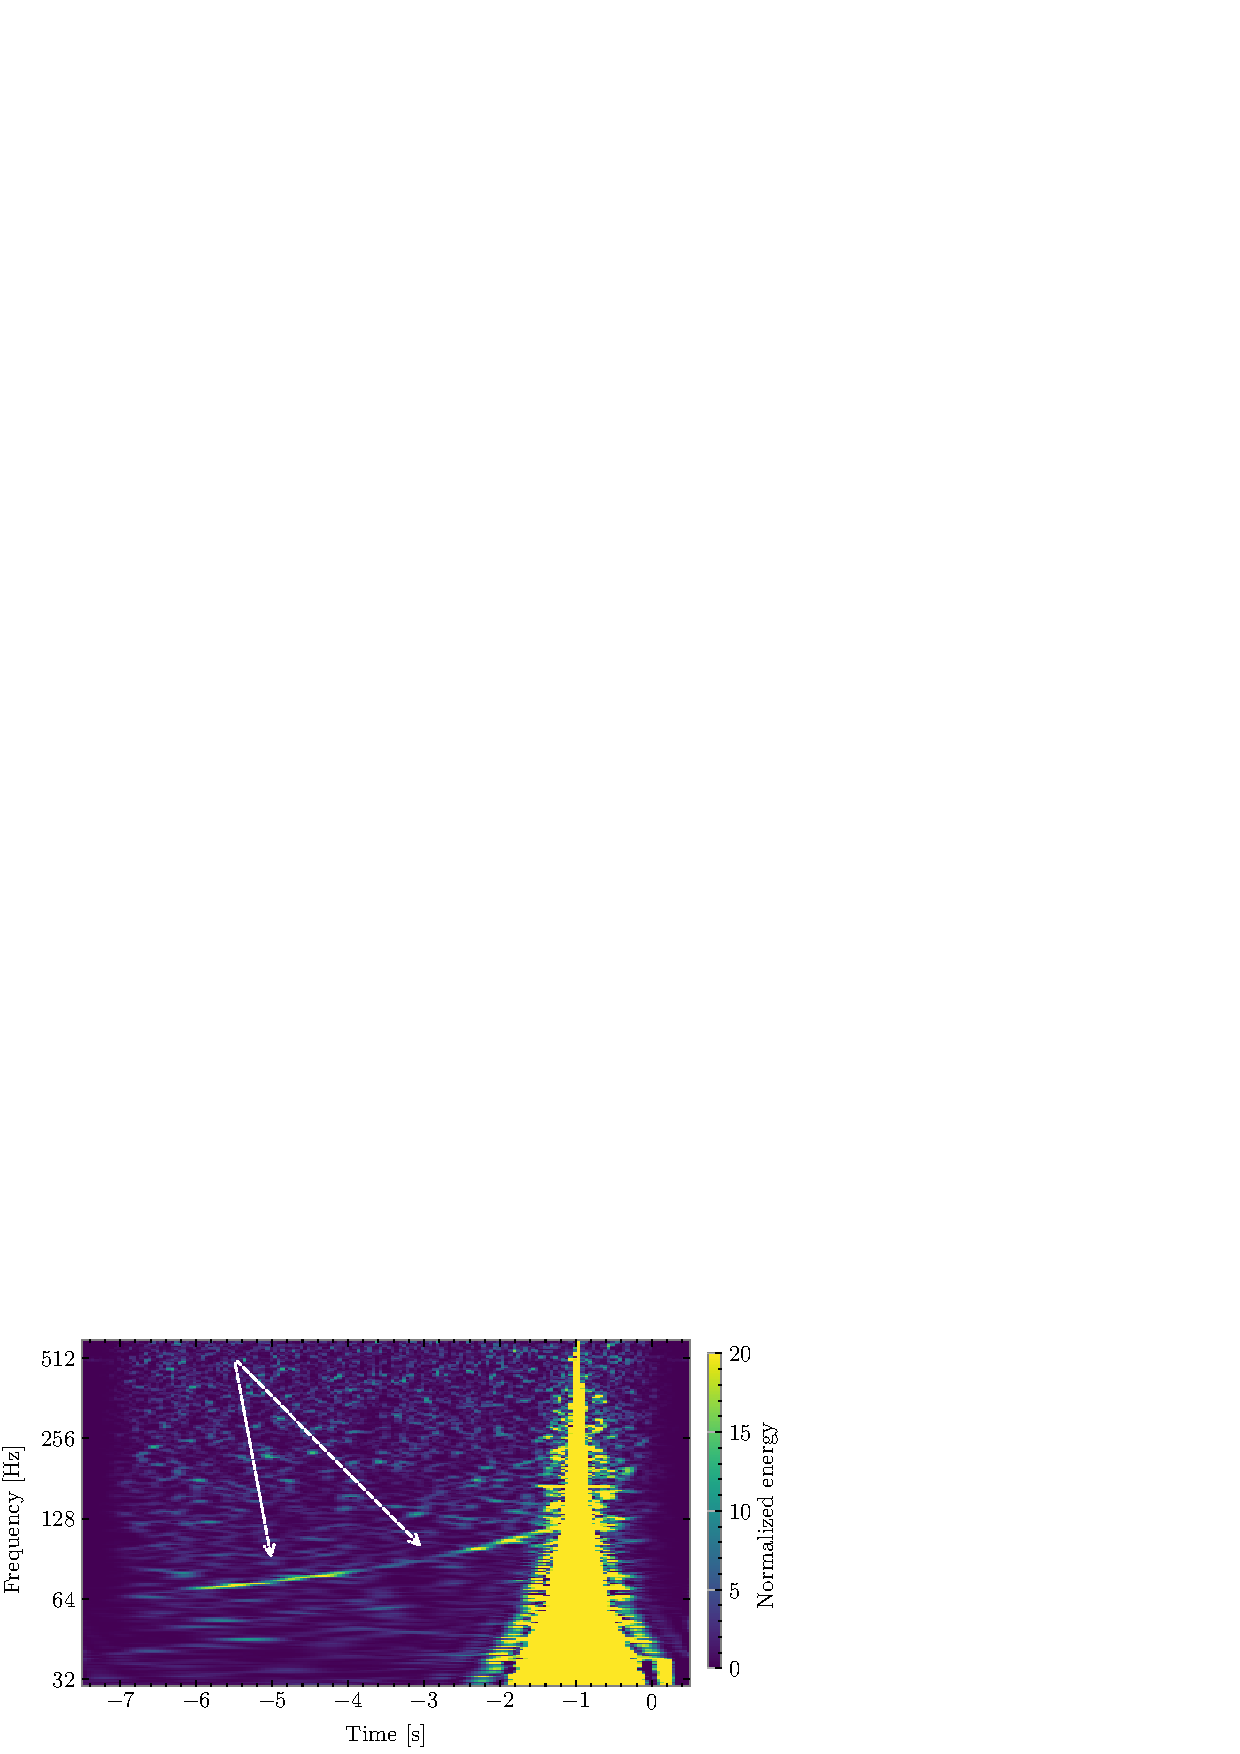
\includegraphics[width=12cm]{../figures/gw170817scan.png}
    \caption{A loud glitch overlapping with the binary neutron star signal, GW170817, in LIGO-Livingston interferometer. Dashed white arrows are added to help reader trace the signal.}
    \label{fig:bns_scan}
\end{figure}
A case where theoretical models do not exist can be made for instrumental noise transients or \textit{glitches}. While the background noise in the GW detectors is assumed to be Gaussian and stationary, occurance of a glitch violates this assumption. As most of our physics inferences hinges on the assumption that background noise is Gaussian-stationry, a violation of it could corrupt the inferences. Depending on the time of occurance, glitches can be problematc in two ways,
\begin{itemize}

\item \textit{Glitches overlapping with a GW signal.} Glitches occuring near a GW signal could corrupt the measurements of its source parameters. Therefore, it becomes necessary to carefully subtract the glitch without the contaminating the signal, \textit{before} we measure the source parameters. The first detection of a GW signal from merger of two neutron star (GW170817) is an example of this kind (Figure~\ref{fig:bns_scan}).
\begin{figure}
    \centering
    \includegraphics[width=12cm]{../figures/thesis-plot_highmass_blip_qscan.png}
    \caption{\textit{Left:} A GW signal emmited by a BBH merger with total mass of $176 M_{\odot}$. \textit{Right:} An isolated blip glitch.}
    \label{fig:bbh_blip}
\end{figure} 
\item \textit{Isolated glitches.} The ones not overlapping with a GW signal, increase the false alarm rate of GW detections since some glitches look similar to a GW signal. For example, the blip glitches have similar time-frequency morphology as GW signals from high-mass BBH mergers [FIXME: Heavy BBH and glitch comparison figure]. It becomes important to identify and veto glitchy data from the analysis to reduce false alarms.
\end{itemize} 


Glitches could be caused by instrumental (control systems, scattered light) or environmental (earthquakes, wind, anthropogenic) factors, though their origins often remain unknown in many cases [FIXME: pictures of glitches]. Thefore, it is not possible to devise a theoretical model for glitches in most cases. We need to rely on the unmodelled approach to reconstruct and subtract glitches. 

\iffalse
A case where theoretical model is expensive to simulate can be made for GW signals from the core collapse of a supernova. A case where theoretical models are not mature enough can be made for the echoes of GW signal. Why do we still do on-source PSD estimation? 
\fi

\section{Transdimensional Sampling Algorithms}
When performing unmodelled reconstruction, the dimensionality of the parameter space of $\vec{\theta}$ is unknown, in contrast to the modelled reconstruction explained in chapter~\ref{ch:gwpe}. While the Bayesian framework, GW likelihood, and Bayesian approximation still remain robust, the Nested sampling algorithm from previous chapter is not a suitable for the problem at hand. Here, we review a transdimensional algorithm that is routienly used to explore a variable dimensional parameter space. Let us define a few standard quantites which formulate building blocks of the algorithm. 
\subsection{Morlet-Gabor wavelets}
\begin{figure}
    \centering
    \includegraphics[width=12cm]{../figures/morlet_gabour.pdf}
    \caption{Morlet-Gabour wavelet in time (left) and frequency (right) domain}
    \label{fig:mg_wav}
\end{figure}
When performing unmodelled reconstruction, we use Morlet-Gabor wavelets as bases functions. It can be expressed in time domain as
\begin{equation}
    \label{eq:wavelet}
    \vec{\psi}(t; A, Q, t_0, f_0, \phi_0) = A~e^{-\frac{(t-t_0)^2}{2\tau^2}}~\sin{\left(2{\pi}f_0(t-t_0) + \phi_0\right)},
\end{equation}
where $t$ denotes time, $A$ denotes amplitude, $\tau = Q/(2{\pi}f_0)$ denotes the quality factor that controls the spread of the wavelet, $\phi_0$ denotes inital phase, $t_0$ and $f_0$ respectively correspond to time and frequency at the peak of the amplitude. In Figure~\ref{fig:mg_wav}, we show a time (left) and frequency (right) domain representation of a wavelet with parameters $Q = 20$, $t_0=1$ seconds, and $f_0 = 40$ Hz. 

Morlet-Gabor wavelets are sutible for the problem at hand because glitches $(\vec{g})$ we want to reconstruct can be expressed as linear combination of $N$ wavelets [BayesWave first paper],
\begin{equation}
    \vec{g}(t; \vec{\theta}) = \sum_{k = 0}^{N} \vec{\psi}_k(t; \vec{\theta}_k),
\end{equation}
where $\vec{\theta}$ is set of $N\times5$ parameters since each $\vec{\psi}_k$ needs 5 model parameters shown in Eq.~\eqref{eq:wavelet}. A desirable feature is that Morlet-Gabor wavelets preserve shape when switching between time-frequency domains and they have a simple analytic expression in both domains. FIXME: There is an undesirable property which is that the wavelets are not orthogonal. 

Besides ${\vec{\theta}}$, here $N$ itself is an unknown parameter therefore the dimensionality of the parameter space we want to explore is also unknown. The transdimensional algorithm used to tackle this problem is an extension of the Markov chain Monte Carlo methods. 

\subsection{Markov chain Monte Carlo}
Markov chain Monte Carlo (MCMC) is a subclass of Monte Carlo methods, a class of computational methods that rely on repeated random sampling to address the problem. Markov chain in particular refers to an iterative process where the probability  of accepting a proposal at $t^{\mathrm{th}}$ iteration depends only on the point from previous iteration. If we denote the probability by $p_t$, 

\begin{equation}
p_t(\vec{\theta}') = \int \mathrm{d}\vec{\theta}_{t-1}~T(\vec{\theta}', \vec{\theta}_{t-1})~\vec{\theta}_{t-1}
\end{equation}
where $\vec{\theta}'$ is the proposed point and $\vec{\theta}_{t-1}$ is the point from previous iteration and $T$ is the transition probability. Standard MCMC algorithms aim to obtain the samples from posterior probability distribution which is in contrast to the Nested sampling algorithm where the aim is to compute the evidence and posterior distributions are the byproduct. Obtaining the evidence after an MCMC algorithm is terminated requires additional computations. Nevertheless, here we outline one such MCMC algorithm called the Metropolis–Hastings algorithm.
\begin{figure}
    \centering
    \includegraphics[width=8cm]{../figures/markov_chain.pdf}
    \caption{\textit{Bottom:} Progresion of a Markov chain in the parameter space of $\vec{\theta}$. Each arrow represents an iteration, filled dots represent accepted proposal and empty dots represents rejected proposals. \textit{Top:} Probability distribution function constructed from the accepted samples of the Markov chain from the bottom plot.}
    \label{fig:mcmc}
\end{figure}
\subsubsection{Metropolis-Hastings algorithm}
Metropolis-Hastings algorithm makes use of a proposal density function ($\Gamma$) to determine whether a proposal point $\vec{\theta}'$ should be accepted. The probability that a proposal $\vec{\theta}'$ is accepted is given by $\alpha$
\begin{equation}
\alpha = \mathrm{min} \left(1, \frac{p(\vec{\theta}' | \vec{d})}{p(\vec{\theta}_{t-1} | \vec{d})} \frac{\Gamma(\vec{\theta}_{t-1} | \vec{\theta}')}{\Gamma(\vec{\theta}' | \vec{\theta}_{t-1})}\right).  
\end{equation}
If the proposal is accepted, it will become $\vec{\theta}_t$ and the step is repeated. The quantity $\Gamma$ can be a Gaussian distribution or any distribution from which we know how to draw samples. Figure~\ref{fig:mcmc} shows an illustration for the progression of a Markov chain (bottom) and posterior distribution constructed from the accepted samples (top). 

\subsubsection{Computing the evidence}
The evidence when using Metropolis-Hastings algorithm is computed in post-processing. Let us introduce a parameter $T$ which is usually known as temperature
\begin{equation}
    p_T(\vec{\theta} | \vec{d}) \propto p(\vec{d} | \vec{\theta})^{1/T} \pi(\vec{\theta}).
\end{equation}
When $T=1$, the right hand side yields posterior weights and when $T=\infty$, it represents the prior. Samples from all chains with $T>1$ are eventually discarded. Writing the evidence as a function of $\beta \equiv 1/T$ to get,
\begin{equation}
    Z(\beta) = p_{\beta}(\vec{d}) = \int \mathrm{d} \vec{\theta}~p(\vec{d} | \vec{\theta})^{\beta}~\pi(\vec{\theta}).
\end{equation}
Let us operate with log and then take derivative w.r.t. $\beta$ on both sides,
\begin{equation}
    \frac{\mathrm{d}}{\mathrm{d}\beta} \ln{p_{\beta}(\vec{d})} = \left< \ln{p(\vec{d} | \vec{\theta})}\right>_{\beta}
\end{equation}
where $\left<.\right>_{\beta}$ stands for the expectation value with respect to the posterior distribution at temprature $T = 1/\beta$. The log evidence is then computed as
\begin{align}
    \ln{p(\vec{d})} &= \ln{p_{\beta=1}(\vec{d})} \\
    &= \int_0^{1} \frac{d}{d\beta}\ln{p_{\beta}(\vec{d})} + \ln{p_{\beta=0}(\vec{d})} \\
    &= \int_0^{1} \frac{d}{d\beta} \left<\ln{p(\vec{d} | \vec{\theta})}\right>_{\beta} + \ln \int \mathrm{d} \vec{\theta} \pi(\vec{\theta}) \\
    &= \int_0^{1} \frac{d}{d\beta} \left<\ln{p(\vec{d} | \vec{\theta})}\right>_{\beta} \\
    &\approx \sum_{\beta = 1/T_{\mathrm{max}}}^{1} \Delta \beta \left<\ln{p(\vec{d} | \vec{\theta})}\right>_{\beta}
\end{align}
Hence, the expectation value of the log-likelihood with respect to the posterior distribution integrated over the temprature range leads to the evidence.

\subsubsection{Limitations of Metropolis-Hastings algorithm}
Indeed, the efficieny of this algorithm depends on the choice of $Q$. In addition, each chain is started at random point and we need to discard certain number of iterations at the beginning so that the dependence on the starting point is lost. This period is called the \textit{burn-in} period which again depends on the choice of $Q$. Moreover, adjcent samples for a given chain maybe correlated which is undesirable. We can choose to store the samples every $n^{\mathrm{th}}$ iterations to mitigate this issue, where n is greater then or equal to the autocorrelation time of the chain. This process is often called thinning.

\subsection{Jumping between dimensions}

\subsubsection{Limitations}

\section{Glitches overlapping with the signals in the Einstein Telescope era}
If we are too aggressive subtracting, one can end up removing part of the signal. If we are too conservative, we may leave behind part of the glitch which can masquarade as signs of new physics. 
